\documentclass[10pt,twocolumn]{article}

\usepackage{times}
\usepackage{fullpage}

\usepackage{booktabs}  % for \midrule
%\usepackage{subfigure}
\usepackage{balance}
\usepackage{graphicx}
\usepackage{xspace}
%\usepackage{pslatex}
%\usepackage{pifont}
%\usepackage{multirow}
%\usepackage{array}
%\usepackage{booktabs}
%\usepackage{cite}
\usepackage{url}
%\usepackage{cancel}
\usepackage{color,colortbl}
%\usepackage{microtype}
%\usepackage{textcomp}% http://ctan.org/pkg/textcomp
\usepackage{tabularx}
\usepackage{framed}
\usepackage[]{algorithm2e}
\SetAlFnt{\small}
\SetAlCapFnt{\small}
\usepackage{algorithmic}

\usepackage{listings}
%\usepackage{scrextend}
%\usepackage{mathtools}
\usepackage{pbox}

\let\labelindent\relax
\usepackage{enumitem}

\usepackage{tikz}
\usetikzlibrary{arrows,automata}
\usetikzlibrary{calc,positioning}
\usepackage{lipsum,adjustbox}

%\usepackage{tikz}
%\usepackage{decorations.pathmorphing}
%\usepackage{assymb}

\usepackage[labelfont=bf]{caption}

%\theoremstyle{plain}
\newtheorem{theorem}{\bf{Theorem}}%[section]
\newtheorem{lemma}[theorem]{\bf{Lemma}}
\newtheorem{corollary}[theorem]{\bf{Corollary}}
\newtheorem{proofl}[theorem]{\bf{Proof}}
\newtheorem{proposition}[theorem]{\bf{Proposition}}

%\theoremstyle{definition}
\newtheorem{definition}{\bf{Definition}}%[section]
\newtheorem{observation}{\bf{Observation}}%[section] 

%\theoremstyle{remark}
\newtheorem{example}{\bf{Example}}
\newtheorem{notation}{\bf{Notation}}
\newtheorem{fact}{\bf{Fact}}

\usepackage{listings}
%%\usepackage{listings-golang}
\usepackage{color}

%\usepackage{sectsty}
%\sectionfont{\fontsize{12}{15}\selectfont}


\newcommand\mypara[1]{\vspace{.3em}\noindent\textbf{#1}}
\newcommand{\urlwofont}[1]{\urlstyle{same}\url{#1}}


%%%%%%%%%%%%%%%%%%%%%%%%%%%%%%%%%%%%%%%%
% Useful reviewing/feedback annotations
\usepackage{ifthen}
%\usepackage[normalem]{ulem} % for \sout
%\usepackage{xcolor}
%\usepackage{amssymb}

\newcommand{\ra}{$\rightarrow$}
\newboolean{showedits}
\setboolean{showedits}{true} % toggle to show or hide edits
\ifthenelse{\boolean{showedits}}
{
	\newcommand{\ugh}[1]{\textcolor{red}{\uwave{#1}}} % please rephrase
	\newcommand{\ins}[1]{\textcolor{blue}{\uline{#1}}} % please insert
	\newcommand{\del}[1]{\textcolor{red}{\sout{#1}}} % please delete
	\newcommand{\chg}[2]{\textcolor{red}{\sout{#1}}{\ra}\textcolor{blue}{\uline{#2}}} % please change
}{
	\newcommand{\ugh}[1]{#1} % please rephrase
	\newcommand{\ins}[1]{#1} % please insert
	\newcommand{\del}[1]{} % please delete
	\newcommand{\chg}[2]{#2}
}

\newboolean{showcomments}
\setboolean{showcomments}{true}
%\setboolean{showcomments}{false}
\newcommand{\id}[1]{$-$Id: scgPaper.tex 32478 2010-04-29 09:11:32Z oscar $-$}
\newcommand{\yellowbox}[1]{\fcolorbox{gray}{yellow}{\bfseries\sffamily\scriptsize#1}}
\newcommand{\triangles}[1]{{\sf\small$\blacktriangleright$\textit{#1}$\blacktriangleleft$}}
\ifthenelse{\boolean{showcomments}}
%{\newcommand{\nb}[2]{{\yellowbox{#1}\triangles{#2}}}
{\newcommand{\nbc}[3]{
 {\colorbox{#3}{\bfseries\sffamily\scriptsize\textcolor{white}{#1}}}
 {\textcolor{#3}{\sf\small$\blacktriangleright$\textit{#2}$\blacktriangleleft$}}}
 \newcommand{\version}{\emph{\scriptsize\id}}}
{\newcommand{\nbc}[3]{}
 \renewcommand{\ugh}[1]{#1} % please rephrase
 \renewcommand{\ins}[1]{#1} % please insert
 \renewcommand{\del}[1]{} % please delete
 \renewcommand{\chg}[2]{#2} % please change
 \newcommand{\version}{}}
\newcommand{\nb}[2]{\nbc{#1}{#2}{orange}}

\definecolor{ibcolor}{rgb}{0.4,0.6,0.2}
\newcommand\iv[1]{\nbc{IB}{#1}{ibcolor}}
\usepackage{wasysym}
\newcommand\yesml[1]{\nbc{ML {\textcolor{yellow}\sun}}{#1}{mircolor}}

\definecolor{sgcolor}{rgb}{0.2,0.0,0.5}
\newcommand\sg[1]{\nbc{SG}{#1}{sgcolor}}

\definecolor{samcolor}{rgb}{0.2,0.4,0.2}
\newcommand\sam[1]{\nbc{SC}{#1}{samcolor}}

\definecolor{hccolor}{rgb}{0.21,0.54,0.84}
\newcommand\hc[1]{\nbc{HC}{#1}{hccolor}}

\definecolor{ideacolor}{rgb}{1.0,0,0.5}
\newcommand\idea[1]{\nbc{IDEA}{#1}{ideacolor}}


\definecolor{abstractcolor}{rgb}{0.0,0.5,1.0}
\newcommand\rabstract[1]{\nbc{ABSTRACT}{#1}{abstractcolor}}

\definecolor{introcolor}{rgb}{0.0,1.0,0.5}
\newcommand\rintro[1]{\nbc{INTRO}{#1}{introcolor}}

\definecolor{papercolor}{rgb}{1.0,1.0,0.0}
\newcommand\rpaper[1]{\nbc{PAPER}{#1}{papercolor}}

\definecolor{multicolor}{rgb}{1.0,0,0}
\newcommand\rmulti[1]{\nbc{MULTI}{#1}{multicolor}}

% Todo Command
\definecolor{todocolor}{rgb}{0.9,0.1,0.1}
\newcommand{\todo}[1]{\nbc{TODO}{#1}{todocolor}}


%%%%%%%%%%%%%%%%%%%%%%%%%%%%%%%%%%%%%%%%


\begin{document}

\title{In-network Contention Resolution for Disaggregated Memory}
%\author{WORDS '21 Submission \#3}
\author{Stewart Grant and Alex C. Snoeren\\ UC San Diego}
\date{}

\maketitle

\section*{Abstract}

Passive remote memory remains the holy grail of disaggregation.  Most
existing systems for disaggregated memory either use remote memory
simply as a backing store, or design special-purpose data structures
that require some amount of processing co-resident with the remote
memory to manage and apply updates.  The few proposals for truly
passive remote memory perform well only with read-mostly workloads,
rapidly deteriorating in the face of even low levels of write
contention.  We propose to leverage in-network devices (specifically,
a programmable top-of-rack switch) to serialize remote memory accesses
and resolve any write conflicts in flight.  Our prototype is able to
completely avoid write contention in the recently published Clover
disaggregated key/value store, delivering a performance boost of
almost 50\% on our testbed under a mixed read/write workload.

\section{Introduction}

There has been tremendous interest in resource disaggregation in
recent years, with both academic and industrial researchers chasing
the potential for increased scalability, power efficiency, and cost
savings~\cite{blade-server,fastswap,rethinking,the-machine,requirements,clio-arxiv,firebox,leap,zombieland,storm,aifm,legoos,supernic}.
By physically separating compute from storage across a network, it is
possible to dynamically adjust hardware resource allocations to suit
changing workloads.  Considerable headway has been made at higher
levels of the storage hierarchy; published and even production systems
support remoting spinning disks, SSDs, and modern non-volatile
memory technologies~\cite{decible}.  Remote primary storage---a.k.a.
memory pooling---remains a fundamental challenge, however, due to the
orders-of-magnitude disparity between main-board access latency and
even intra-rack round trips.

%Resource disaggregation is an architectural paradigm which separates
%disk, CPU and memory over a network. The goal of this architecture is
%to enable extreme flexibility in terms of machine composition.  For
%example a systems memory capacity can be dynamically apportioned by
%reconfiguration, rather than by manually changing the physical
%components of a single machine. It is now common for disks (HHD and
%SSD) to be disaggregated from CPU and memory. SSDs are comparatively
%easier to disaggregated than main memory as their access latencies are
%on the order of 10's of microseconds which amortizes the network round
%trip cost.

%Local memory latency is around 50ns. The cost of accessing memory over the
%network is on the order of 1us -- approximately a 20x overhead. This order of
%magnitude difference in latency makes hiding remote memory accesses a hard
%problem.  

The hardware community has made great strides in closing the latency
gap via novel technologies like silicon photonics and new rack-scale
interconnects, but commercially available options remain significantly
slower than on-board options.  Concretely, while industrial consortia
have proposed cache-coherent memory technologies~\cite{genz,cxl} that
would dramatically lower access latencies, currently available
interconnects based on RDMA~\cite{infiniband-spec}
%%
%\todo{distinguish CXL 200-500ns latencies have been proposed}
%%
remain on the order of 20$\times$ slower than a local access (e.g.,
50~ns local versus 1~$\mu$s remote).  As a result, despite the fact
that current-generation memory transport technologies provide the
ability to directly execute requests like read, write, and compare and
swap on remote host memory through the use of RDMA-capable
NICs~\cite{connectx}, SoCs~\cite{cavium}, FPGA
SmartNICs~\cite{corundum,kv-direct}, or DPUs~\cite{fungible}, most
existing systems coordinate with a remote CPU on the socket at which
the DMA is being performed to assist with
serialization~\cite{cliquemap,erpc,herd,sonuma,storm}.
%%


%% % and Omni-Path~\cite{omni-path}. // omni-path is dead now % 
%Each protocol, while distinct, meets approximately the same requirements,
%reliable access to byte addressable remote memory with low latency and high
%throughput.

%% it would be nice to Cite SUPERNIC and CLIO here but I'm not sure it makes
%sense untill it's published at a major venue
%%Clio~\cite{clio-arxiv}
%%todo ask alex about the archive reference
%%todo do a quick read of how DMA is dealt with on the other interconnects

In the absence of a general-purpose CPU located alongside remote
memory, it falls to each individual client to ensure that its reads
and writes are serialized, usually by leveraging expensive
hardware-provided atomic operations at the server like
compare-and-swap (CAS)~\cite{design-guidelines} as the latencies
involved in client-side coordination are prohibitive.  As a result,
most existing systems simply partition memory completely and forgo
sharing~\cite{reigons,fastswap,legoos}.
%%
%The few published systems that provide fully passive remote memory
%target scenarios involving read-heavy workloads~\cite{clover}, client
%colocation~\cite{sherman}, or memory-inefficient
%datastructures~\cite{race} \textbf{XXX:Need to say more} where the
%costs of conflict detection and resolution can be effectively
%amortized.
%
The few published systems that do support shared access mediate
requests to specialized data structures~\cite{clover,sherman}.

For example, Sherman, a write-optimized
B+Tree~\cite{sherman} places its locks in NIC memory at the server to
avoid crossing the remote PCIe bus.
%, resulting in 3$\times$ higher throughput.
Clover~\cite{clover} implements a hash table that
supports lock-less reads; concurrent writes are supported through a
client-driven optimistic concurrency protocol.  Despite their clever
designs, however, both approaches simply delay the inevitable:
%%
Sherman's NIC-based locks are subject to significant hardware limits
imposed by the CAS operation required to enforce serialization.
Similarly, Clover's client-based recovery scheme quickly becomes cost
prohibitive when faced with non-trivial levels of write contention.
%
%it is repeatedly executed on a single
%address (Lock acquire and release). Further, Sherman requires that cliques of
%clients are colocated to resolve most contention based conflicts locally.
%%
% CAS instructions are only executed to commit
%writes and never land on the same address twice - effectively bypassing the
%single address limits of CAS.
%%
%While highly scalable for read-heavy workloads,  This

We argue that these shortcomings are not unique to the particular
systems, but rather fundamental to any approach that implements
distributed conflict resolution.
%
%% minimize conflicts by caching  metadata about the
%% location of the latest writes and reads while also make use of a
%% remote data structures which allows for lock-less reads. In the case of
%% highly contended resources however the performance of clover
%% diminishes sharply due to an increased number of atomic locking
%% operations required on writes.
%
The obvious alternative is to deploy a centralized memory controller
(e.g., a CXL 2.0 switch) that can serve as a serialization point and
ensure all races are resolved before accessing memory, but effective
realization of such a design has proven elusive.  While many proposals
exist, none of them have yet been implemented in commercially
available hardware.  More to the point, such designs are inherently
unscalable as they require all accesses to be managed by the
controller, rather than forwarded directly between the client and
relevant server.

In this work we make the observation that such a serialization point
already exists in today's rack-scale disaggregated deployments: the
top-of-rack switch.  We propose to leverage the capabilities of modern
programmable switches to cache sufficient information about in-flight
requests to transparently detect and resolve conflicts before they
occur.  Unlike a centralized memory controller, however,
our serializer does not need to operate on---or even maintain state for---all
remote memory requests.  First, it only needs to address actual conflicts
and can avoid the unnecessary costs of enforcing ordering among
unrelated requests.  Second, in deployment scenarios where it may
lack the resources to track all requests, our serializer can serve as a
performance-enhancing proxy: when deployed alongside client-based
conflict resolution techniques, it can allow even conflicting requests
to pass through unmodified without jeopardizing safety while
decreasing the frequency of conflict resolution.

We present {\sword}, an on-path serializer
%(implemented either
%directly on the top-of-rack switch or an attached
%middle box~\cite{disandapp})
that dramatically improves the performance of remote memory systems
that support write sharing.  Like all ToRs, {\sword} imposes a
globally observable total order on memory requests (i.e., packets)
within a rack.  In scenarios where {\sword} has the resources to
explicitly manage RDMA connections, it can enforce per-server ordering
at the ToR and remove the expensive CAS operations from all in-flight
packets, avoiding their associated performance bottlenecks entirely.
More generally, however, {\sword} can be deployed alongside an
underlying optimistic concurrency scheme: remote memory operations
remain guarded to ensure that clients can detect and recover from
conflicts of which {\sword} may not be aware.  Instead, because
{\sword} understands the disaggregated memory protocol, it can keep a
cache of recent operations to adjust subsequent requests whose
guards it knows are doomed to fail.  In such cases,
%If suitably provisioned (i.e., it has the
%appropriate metadata cached),
it modifies requests in
flight to account for the preceding operations and decrease the
likelihood the guard will trip.

We prototype {\sword} in two scenarios using a rack of servers
equipped with ConnectX-5 RoCE-enabled NICs.  First, we use a
DPDK-based implementation to replace CAS requests in flight with
standard RDMA verbs, allowing systems like Sherman to overcome the
hardware-imposed limit on atomic requests per queue pair.  Second, we
implement a lightweight version of \sword\ on a P4 programmable switch
to accelerate Clover's optimistic concurrency protocol. Our evaluation
shows that {\sword} dramatically increases the performance of Clover
in the presence of write contention: Under a 50:50 read-write
workload, throughput rises by almost 35$\times$, tail latency drops by
over 300$\times$ and bandwidth usage drops by 16$\times$.

%% Using RDMA transport information and clover specific application
%% knowledge all reads and writes to contended areas are totally ordered
%% in the network. Specifically all reads and writes to the same keys are
%% multiplexed to the same queue pairs, by utilizing the RDMA ordering
%% requirements of QP's reads and writes require no expensive locks and
%% can flow at line rate to remote memory. This ordering requires a
%% number in band adjustments to the RDMA protocol in order to
%% interoperable with commodity hardware. QP state must be maintained in
%% network, specifically the sequence numbers of multiplexed requests, so
%% that response packets can be demultiplexes back to their original
%% connections. Small adjustments such as generating ACKs for collapsed
%% requests is also required. We demonstrate that these algorithms are
%% implementable in network at little cost with a DPDK prototype. We
%% measure that ~\todo{we achieve a ?X improvement in performance using
%%   only XMB of in network state, and ?X performance improvement in
%%   highly contested settings with full use of system memory}.

\section{Background}

While our insight and approach is general, in order to demonstrate its
practicality we prototype it in the context of Clover~\cite{clover}, a
disaggregated key/value store.  Hence, we begin with a brief overview
of the relevant aspects of Clover's design for the uninitiated.

\subsection{Append-only updates}

\begin{figure}
    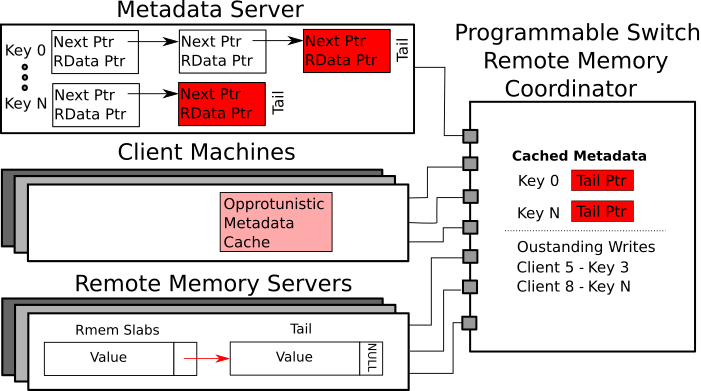
\includegraphics[width=0.45\textwidth]{fig/overview_2.png}
%%
    \caption{ System overview, Metadata, client, and Remote Memory
    servers are Clover components. Our remote memory coordinator is
    located on a centralized TOR interconnecting the clover components.
    }
%%
    \label{fig:overview} 
\end{figure}

Clover maximizes performance by storing data in a versioned list, dubbed a
\emph{chain} by the authors, which allows for fully asynchronous non-blocking
reads and $O(1)$ writes which succeed opportunistically. Writes are issued by
clients as atomic append operations to the end of the chain, the structure of
which is illustrated in Figure~\ref{fig:overview}. Each entry in the chain
contains a pointer to the next entry with the pointer at the tail of the
chain set to \texttt{NULL}. Clients keep cached pointers to the current tail of the
chain for each key allowing them to issue locf-free RDMA reads directly to

passive remote memory servers using the address they believe to be the
current tail. Clients can independently confirm their reads are
fresh by ensuring the value returned has a \texttt{NULL} next-update pointer.

Write (i.e., append-to-tail) operations, on the other hand, require two steps
in the common case. First a writer issues a lock-free RDMA write to store the
new value update to an uncontended portion of remote memory. The
second operation optimistically attempts to make the update globally visible
by atomically committing it to the end of the chain. Specifically, the writer
issues an RDMA compare-and-swap (\texttt{c\&s}) operation to the old tail to replace
its (presumably still \texttt{NULL}) next-update pointer with the address of the
new value. If successful, it then updates the metadata sever with
the new end-of-chain address.
%(as any concurrent writes to the same location will fail the comparison).

%% This operation ensures that the next
%% write to the data structure writes to the tail of the linked list.
%% This operation requires two steps.

The Clover authors compare their opportunistic approach with a variety
of different system architectures including one which centralizes
metadata on the datapath (pDPM-central). They find that their
opportunistic approach achieves extremely high throughput on
read-heavy workloads, performing similarly to raw RDMA reads.  In
contrast pDPM-central bottlenecks at far lower throughput.  In the
presence of writes Clover's throughput decreases due to contention
while the performance of pDPM-central remains the same as it resolves all
concurrent write conflicts in the data path.



\subsection{Conflict handling}

If multiple clients attempt to update the value concurrently, each will
succeed in their first write to their private region of remote memory but
then issue conflicting RDMA \texttt{c\&s} operations to the end of the shared chain.
The race is resolved at the remote memory location of the previous update in
the chain: only the first \texttt{c\&s} operation will succeed; all subsequent
operations will fail because rather than finding a value with a \texttt{NULL}
next-update pointer, they find the now (at best) penultimate value in the
chain which points to the update issued by the client that won the race.
%When concurrent writes update the same key a race occurs to write at the end
%of the chain. Write operations require two separate RDMA transactions that
%must each complete to ensure atomicity.
During this two-RTT operation any concurrent write to the same key will cause
a conflict.

%% The process which lost the race now needs to engage in \textit{Pointer
%% chasing} to find the new tail. It must iterative issue reads of the
%% linked list, step by step until it finds the location of the new tail.


If a client's write---or read---fails because it used a stale tail pointer
the client concurrently requests the new tail address from the metadata
server and iteratively traverses the chain themselves to find the current end
in a processes known as \emph{chain walking}. (It is insufficient to just
consult the metadata server because it is updated lazily.) Failed writers
must then issue a new \texttt{c\&s} operation at the updated end of the chain to
append their pending update. Of course, the reissued \texttt{c\&s} is subject to the
same race condition as many writers may be executing concurrently. This
pointer-chasing reconciliation algorithm must be run independently each time
a conflict occurs.
%The slower writers will fail the guard, and must retry their c\&s operation
%after walking the chain through remote memory or by getting an update from
%the metadata server.
While concurrent read operations will not prevent a write from succeeding, a
reader that loses the race with a \texttt{c\&s} operation will need to issue another
RDMA read to the new address to obtain the updated value. On write-heavy
workloads these race conditions happen frequently
%as illustrated in Figure~\ref{fig:conflicts}, , which leads to a sharp
%decrease in throughput. For highly contested structures, the number of
%retries can grow quickly,
leading to large and unpredictable tail latencies~\cite[Table 2]{clover}.




%\begin{figure}
%    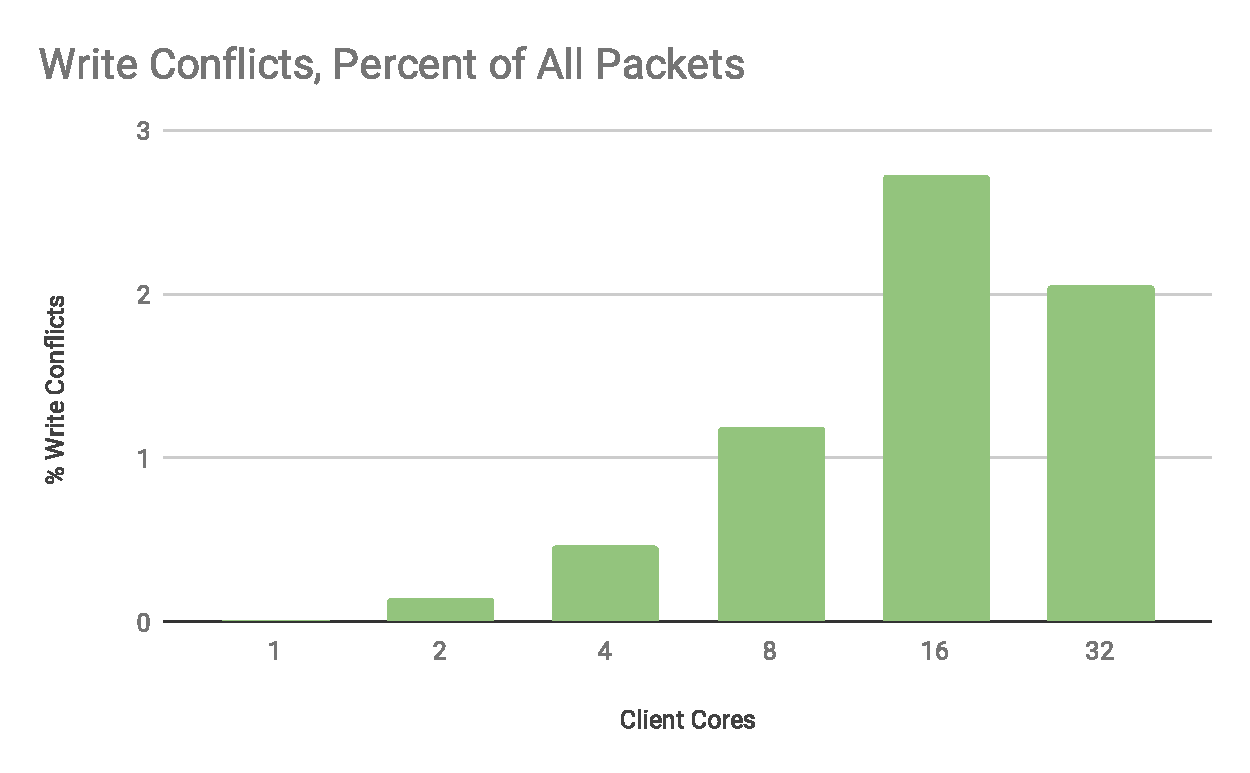
\includegraphics[width=0.45\textwidth]{fig/write_conflicts.pdf}
%    \caption{Clover write conflicts grow with the number of clients
%    (50\% write Zipf 0.99 distribution)\todo{redo with 64 cores and
%    writes only}}
%    \label{fig:conflicts}
%    \vskip -0.5em
%\end{figure}



%% The high level pitch about remote memory.
%Far memory projects typically have a remote CPU which is used to
%coordinate access to remote resources (cite all object systems). In a
%disaggregated system there is no remote CPU, therefore the coordination
%of reads and writes to remote locations must be done locally. For
%performance local caches of remote resources can be used to organize
%access to remote resources. For data structures which require
%consistency this creates a problem as stale caches can lead to data
%structure corruption.


\section{On-path serialization}

Given the overhead of remote conflict resolution and the performance
bottlenecks associated with RDMA hardware serialization, this section
discusses how an on-path serializer can dramatically increase
real-world performance by alleviating both issues.  To ground our
discussion, we address both in the context of Clover, a
state-of-the-art far memory system. First we describe how to
effectively do away with the need for most retries by ``fixing''
operations issued with stale hints in flight.  Second, we show how we
can leverage our ability to rewrite RDMA requests after their ordering
is determined to replace expensive compare-and-swap requests with
simple write verbs and rely upon the semantics of RDMA RC queue pairs
to provide serializability.  Additionally, we can leverage this same
functionality to multiplex independent operations across multiple QP
to improve scalability.

\subsection{System overview}

Any asynchronous data structure which allows for lockless reads and
writes must have a mechanism in place to resolve conflicts. When
memory is close, conflict resolution strategies can make many reads
and writes quickly; in the uncommon case of a conflict, the cost of
resolution is typically amortized by the unlikelihood of the conflict
itself. In the case of far memory the cost of a conflict is severe. In
contrast to opportunistic algorithms in a shared-cache architecture,
in a rack-scale disaggregated system conflicts can be detected at the
top-of-rack switch and resolved in the data path. Our solution,
\sword, leverages programmable ToR switches to allow developers with
knowledge of the disaggregated memory protocol to resolve conflicts
transparently in flight as the operations flow traverse the ToR.

\begin{figure}
\center
  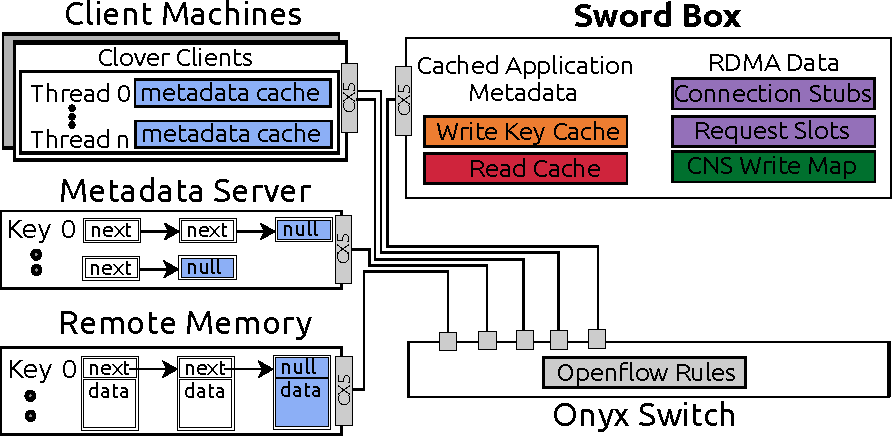
\includegraphics[width=0.45\textwidth]{fig/overview_2.pdf}
  %%
 
\caption{Clients, Metadata and Remote Memory servers are
Clover components. {\sword} is run on a separate server connected to the same ToR.
Routing to {\sword} is effected by adding OpenFlow rules to redirect Clover traffic to \sword.}
%%
\label{fig:overview} \end{figure}

Figure~\ref{fig:overview} shows how {\sword} interacts with the Clover
system.  We envisage {\sword} implemented either as a part of or in-line with
a programmable switch that serves as the top-of-rack (ToR) switch
for all of the memory servers.  Client machines need not be directly
attached to the ToR, although they likely would be in most rack-scale
deployments.  Similarly, the topological location of Clover's metadata
server is irrelevant, but we expect it is also likely connected to the
same switch.  For the purposes of our discussion, we presume that
{\sword} first places all received RDMA requests into a total order
before processing them; likewise responses from a given memory
server are totally ordered before processing.

\subsection{Conflict avoidance}

The single biggest impact an on-path serializer like {\sword} can have
is to dramatically decrease the likelihood of a failed RDMA request due
to a stale hint.  Specifically, because {\sword} can observe and
modify operations as they go by, it can ``correct'' any requests it
knows to be likely to fail.  Note that such replacement is strictly a
performance enhancement---because the requests continue to be
processed by the server as usual, any subsequent reordering will
cause the request to fail (and be retried by Clover), just as
it would have without rewriting.

\subsubsection{Write steering}

Recall that writes (committed with compare-and-swap requests) in
Clover are destined to the presumed tail of a key's linked list, but
the target of any individual RDMA request may be out of date due to
races with concurrent updates.  To prevent such requests from
failing, {\sword} maintains a cache of the location of the most-recent writes
for each key. If a write (CAS request) arrives at {\sword}
destined for a stale virtual address (i.e., an address other than the
one currently cached for that key), {\sword} replaces it with
the cached address.

While conceptually simple, the actual implementation is somewhat
involved due to the design of both Clover and the RDMA protocol and
our desire to remain transparent to both.  Specifically, Clover RDMA
CAS requests do not explicitly specify the operation of which they are
a part.  {\sword} infers the operation by checking the size of the
RDMA request and then extracts the key from the appropriate the
location in the packet.  The key is then used as an index into a
lookup table to find the virtual address of the latest write for that
key.  Our strategy requires only 64 bytes of data per key---the size
of the RDMA virtual address.  Because it modifies the content of the
RDMA request, {\sword} also needs to recompute the RDMA ICRC checksum
to prevent the server from rejecting the request as malformed.

%By
%performing this lookup in the data path all writes succeed regardless
%of how contested the memory address is. \todo{ref fig from words}.

\subsubsection{Read steering}

Reads present a slightly more complicated case. Writes contain the key
to which they pertain---which allows for a table lookup---but Clover's
RDMA read requests only contain the target virtual address and a size.
%When a
%read fails it must be retried, as mentioned earlier reads are
%performed iteratively until the tail of the list is reached, which in
%the case of highly contested keys could be arbitrarily long. Repeating
%reads does not destroy system performance as they are lockless,
%however in terms of client latency each retry adds serious
%latency. What makes handling reads hard is identifying the clover key
%for which the read is for, without additional data in the packet the
%value must be determined another way.
As reads can be for arbitrarily old virtual addresses a naive solution
that stored the lineage of each key would effectively require
caching the entire contents of Clover's metadata server.  Our solution
is to hash the address of each write into an array somewhat larger than
the size of the key space, and store the key along with the address.
Hash collisions are resolved by replacing the old address and key with
the new values, allowing keys with higher update rates to maintain
longer histories in the table. 

When reads arrive {\sword} looks up their destination address in the
table; if the address has a hit the associated key is used to look up
the current tail in the write cache and the RDMA read is redirected to
the cached location.  Should a miss occur---either because the hash
bucket was overwritten by another key, or because the tail address is
not cached---the read is left unmodified.  If it fails to arrive at
the current tail, Clover's default recovery mechanism kicks in and
performs a lookup to the metadata server for the last known address
and the process repeats. We find that by using an array size of
3$\times$ the vast majority of reads succeed first try. One advantage
of this technique is that it is a generalized cache for recent RDMA
reads, and requires little computation to maintain a hot cache. For
performance reasons we forgo heavyweight hash functions and use
the \texttt{murmur3} bit scrambler to attain an approximately even
hash of virtual addresses in only a few cycles.
%---which can likely be
%implemented on programable switch hardware.

\subsection{Enforcing ordering}

The combination of read and write steering dramatically improves the
performance of Clover (as shown in Section~\ref{s:results}), but only
scratches the surface of the potential improvements for far memory
systems.  In particular, if {\sword} is able to ensure that
requests will not be reordered between when it operates on them and
their arrival at a memory server---because, for example, it is
directly connected over a single link---we can leverage the ordering
semantics provided by RDMA queue pairs to completely eliminate data
races.  In that case, there is no need to incur the expense of RDMA
atomic requests; {\sword} can simply replace them with lightweight verbs
to dramatically increase the scalability of a given memory server.
Importantly, this optimization can be applied selectively to only the
set of servers (or keys) for which {\sword} is suitably located
and sufficiently provisioned to manage; Clover operations destined
for other servers and/or keys can be left unmodified---or subject just
to read/write steering as appropriate.

\subsubsection{Connection remapping}

Our key insight is that if all operations---across all client
connections---that share server state are vectored to the same queue
pair, RDMA's ordering semantics will provide sufficient serialization.
In general, the determination of which operations share state is
application specific and requires inspecting each packet, extracting
the relevant pieces of metadata, and vectoring the packet to the
correct connection.  In the particular case of Clover, it suffices to
identify RDMA requests that correspond to requests to read or write
the same key.

%%While removing locking operations is a general principle here we consider a
%%solution for RDMA.  %Different transports with different ordering guarantees
%%would require bespoke solutions.  

The challenge, of course, is that the RDMA specification stipulates
that each client establish its own queue pair with a given server, so
operations for a given key from different clients will arrive on
separate queue pairs.  \sword, then, must interpose on the
full set of queue pairs terminated by a given (set of) server(s) and
vector operations to queue pairs accordingly.

\paragraph{Sequence-space stitching.}

Multiplexing and demultiplexing RDMA requests across established
connections requires a significant amount of care. Requests on a
single connection must have monotonic sequence numbers from both the
sender's and receiver's perspectives. If monotonicity is broken, the
NIC will invoke an expensive go-back-$n$ protocol or issue explicit
congestion notifications. To ensure monotonic sequence numbers on
shared connections {\sword} tracks the outstanding sequence number per QP and
injects the appropriate sequence number into the packet after the
mapping decision has been made.  (Ironically, there is no need to
ensure any particular ordering among requests from separate clients, so
any total ordering suffices.)
%% This monotonic sequence number increment and QP mapping is the
%% serialization point which replaces the use of the RDMA CAS
%% request. As long as a packet is given an atomically incremental
%% sequence number from our middle box and placed on a stateful
%% partitioned connection, it will execute in the same serialized
%% order as if it were protected by a CAS. We are guaranteed this due
%% to the ordering requirements of RDMA reliable connections.

When an RDMA request arrives at {\sword} from a client, it is
mapped to the appropriate queue pair for the relevant key and a
\emph{stub} is stored to aid in mapping the request back, much like a
network address translator (NAT). The stub keeps track of the original
request's sequence number, IP address, MAC address, and queue
pair. Stubs are stored in an array of size $n$ indexed by their
sequence number$\pmod n$ to ensure $O(1)$ lookup when demultiplexing
the response.
%%
In addition to sequence numbers, a \emph{message} sequence number
is used as an RDMA optimization by the memory server NIC. This value
is transmitted as part of the RoCE BTH+ header in the response packet
and corresponds to the highest request number the server has
processed. If this value is wrong in the response packet from the
perspective of the sender (i.e., is less than another message sequence
number previously received by that client), the entire request is
retransmitted.  {\sword} maintains the message sequence number each client
expects to see by keeping track of the number of requests a client has
issued and adding it to the value of the original message sequence
number for that connection.

\paragraph{Request coalescing.}

As an additional complication, {\sword} must deal with the fact
that RoCE coalesces some ACKs as an optimization.  In particular
multiple RDMA requests can be acknowledged by a single
acknowledgment, in the form of either an ACK, ATOMIC ACK, or Read
Response. This occurs when multiple RDMA requests are processed
concurrently.  Because {\sword} maps requests across connections, some
coalesced acknowledgments may need to be disaggregated from the
clients' perspectives.
%
%A final additional challenge in mapping
%requests, is that receiving NICs can coalesce acknowledgment messages. Given a
%single connection, if two concurrent writes are issued, it is perfectly valid
%for an RDMA NIC to only ACK the second write. This is a challenge when mapping
%requests as a coalesced message might have been for a different sender. In our
%scheme as all requests have mapping stubs stored in the middle box,
{\sword} can detect such conditions by comparing the
acknowledged sequence number to that stored in a client's stub; when a
request is coalesced a gap in the sequence number is observable. In
this case we generate the needed acknowledgment at {\sword} and
insert it into the queue pair.
%While read, and CAS requests can not be
%coalesced, CAS requests mapped to writes can be. In the case of
%coalesced ATOMIC ACKs an atomic ACK is generated in place of the
%coalesced write ACK.



\subsubsection{Atomic replacement} 

Once any potentially conflicting operations are mapped to a single
queue pair, {\sword} is free to replace atomic requests such as
compare-and-swap with lightweight alternatives.  From a RoCEv2 perspective
the per-packet transformation from CAS to write can be applied easily
in the data path.  RoCEv2 CAS and write headers only differ by a few
fields. CAS can be thought of as a special case of a write, where the
write is conditional and the length is preset to 8 bytes.
%%

{\sword} transforms CAS requests to writes by modifying their headers: it
switches the RDMA OP field of the CAS to write, copies the CAS
value to the write payload location, sets the DMA length of the write
to 8, and shrinks the IPv4 length value by 4.  Post modification the RoCEv2
and IPv4 checksums are recalculated.
%so the modified packet will not be
%rejected by the memory side NIC.
The transformation from CAS to write
is deterministic and only requires a few cycles to transform the
header.

On the memory server, the NIC processes the write and responds with a
regular, write ACK. Once the ACK reaches {\sword} we apply the
inverse transformation from the ACK to an Atomic ACK which the sender
expects to see.  RDMA Atomic ACK headers are very similar to regular
ACKs with the only difference being that the atomic contains the
original data from the memory location of the CAS. This original data
is missing due to the transformation so we inject a value which
indicates success to the sender.
%%
This value is application specific; in Clover's case 64 zero bits
indicate success.  In other cases it may be necessary to store the
value in the request stub at {\sword}.

%Transforming CAS to
%write does nothing to disturb the RDMA protocol, as both the sender
%and receiver side NIC are oblivious.  However, the guarantees the
%atomic provides, such as write serialization and the prevention of
%read tearing has been lost. To prevent arbitrary corruption of data
%the serialization point must be placed somewhere else. Our approach is
%to detect conflicts in network, and utilize the in order delivery
%guarantees of RDMA reliable connections to ensure safe and serialized
%requests.



\section{Evaluation}
\label{s:results}

%We use two distinct prototype implementations to demonstrate the
%potential performance benefits \sword\ can provide.

We use our DPDK implementation to perform a micro-benchmark where we explicitly
manage RDMA connections to remove the atomic operations used by Sherman's
locking mechanism.  We use the P4 implementation installed on a programmable
switch to show the impact of in-flight conflict resolution at rack scale in
Clover.

%We discuss the relative impact of each of our techniques across
%various workloads, and demonstrate that replacing compare-and-swap
%requests with writes eliminates hardware bottlenecks.

\subsection{Testbed} 

Our testbed consists of a rack of nine identical machines equipped
with two Intel Xeon E5-2640 CPUs and 256 GB of main memory evenly
spread across the NUMA domains. Each server is equipped with an
NVIDIA Mellanox ConnectX-5 100-Gbps NIC installed in a 16x PCIe slot and connected to a 100-Gbps ToR.  Our DPDK-based
micro-benchmarks use only three machines: a load generator, a memory
server, and a machine hosting our DPDK implementation of {\sword}.
The load generator is configured with default routing settings---it
sends traffic directly to the memory server.  We install OpenFlow
rules on a Mellanox Onyx switch to redirect the traffic to the DPDK
box.  For the P4-based Clover experiments, we replace the Onyx switch
with an Edgecore Wedge-100 programmable switch running \sword.
%Figure~\ref{fig:overview} shows the layout of our testbed.
We configure one server as a Clover memory server, one as a metadata
server, and the remaining seven as Clover clients.

%\subsection{FUSEE}

%FUSEE is a recent RDMA-based disaggregated memory system
%with similar design principles to clover~\cite{fusee}. Fusee
%is built on RACE hashing~\cite{race}, and uses a one-sided
%snapshot algorithm for replication. Unlike Clover, FUSEE
%manages it's metadata only using one sided operations
%increasing the complexity of its updates. FUSEE is also not
%designed for persistent memory, updates are performed
%opportunistically, and the \textit{first client to finish}
%succeeds in making an update.

\subsection{Atomic replacement}

\begin{figure}[t]
  \center
    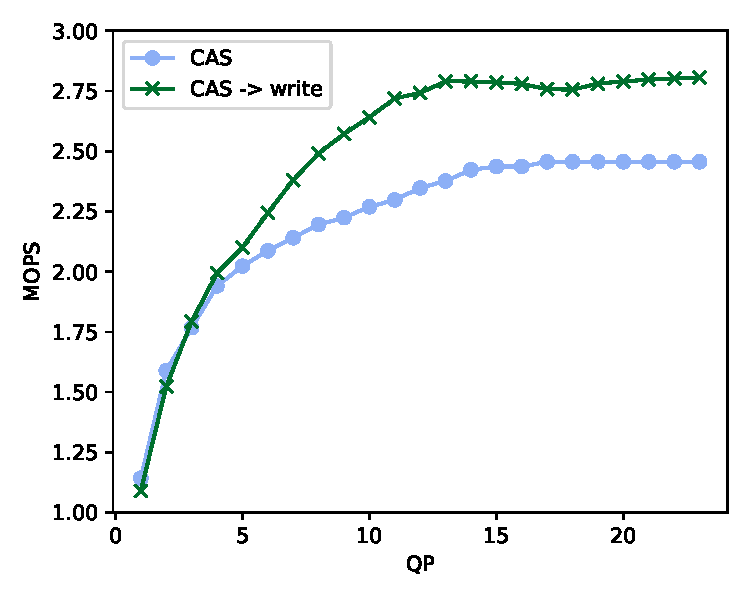
\includegraphics[width=0.99\textwidth]{fig/cas_vs_swap.pdf}
%  \vskip -0.5em
    \caption{Throughput of conflicting CAS and rewritten CAS requests as a function of client threads/QPs.}
    \label{fig:cas_vs_swap}
      \vskip -1em
\end{figure}

\begin{figure*}
  \center
    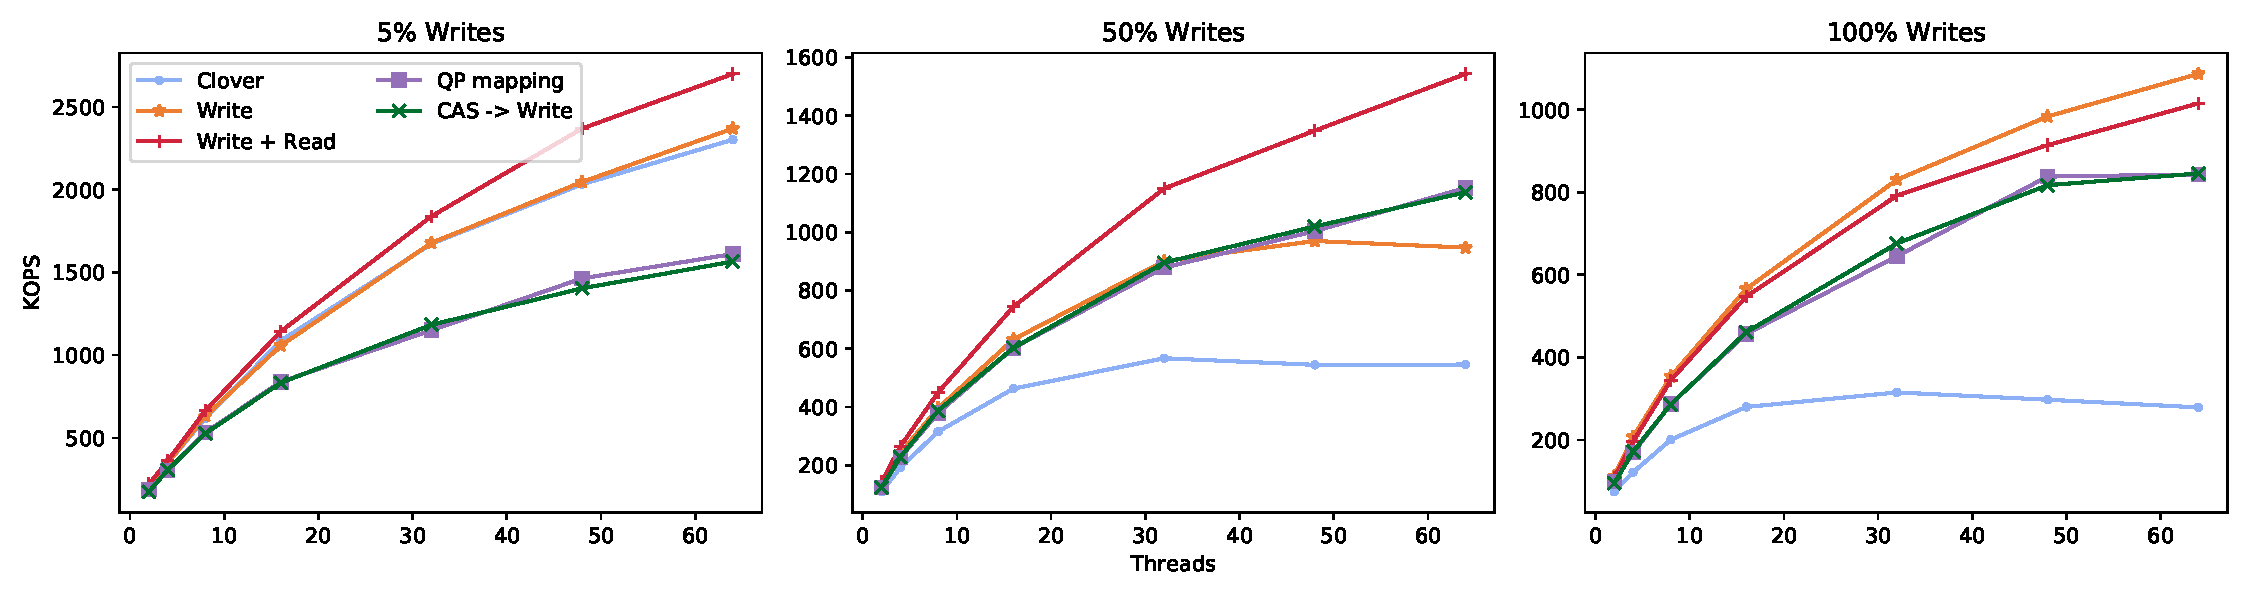
\includegraphics[width=1.0\textwidth]{fig/full_system_performance.pdf}
%  \vskip -0.5em
    \caption{Steering applied to Clover with 128-byte objects across 4 YCSB
    benchmarks. The percentage of workload writes increases from left to
    right. \sword\ throughput relative to Clover is 1.0, 2.8, 32, and 46$\times$ respectively.}
    \label{fig:full_system_performance}
%      \vskip -0.5em
\end{figure*}

We show that \sword\ is able to overcome the NIC hardware
bottleneck by replacing CAS operations with writes
serialized on a given RC by running a micro-benchmark that
focuses exclusively on CAS performance. Specifically, we
extract the CAS request from Sherman's lock operation and
repeatedly generate it from one client to a single memory
server (while routing it through {\sword} using OpenFlow
rules).
%Here we remove clover from the mix and run a simple
%benchmark of RDMA CAS operations between two servers.
%\sword is routed to via a different set of OpenFlow rules.
Each client thread is bound to its own queue pair, and all
client threads issue CAS requests to the same shared virtual
address.  We set the number of cores on the {\sword}
middlebox to 24 so that in our maximal test case each client
thread flows through exactly one middlebox core for the
lowest degree of interference between QP.

%All requests are routed
%through our middlebox.
Figure~\ref{fig:cas_vs_swap} shows the results when all requests are
directed at the same address in the remote server's main memory.  In
the default case (labeled CAS in blue), {\sword} lets CAS requests
flow through without modification, each on their own queue pair.  In
the CAS$\rightarrow$Write (green) configuration {\sword} maps all
client requests to the same QP at the server to ensure serialization
and replaces the CAS operation with a simple write.
%
%all client cores request the same address, and as such all are routed
%onto the same destination QP. Note that this configuration has the
%highest degree of contention for our middlebox as 24 client threads
%must be multiplexed to and from a single client connection. Further
%
%We measure the server throughput in terms of RDMA requests per second as we
%increase contention by adding client threads.
We see a significant increase in performance when \sword\ converts
CAS-guarded requests to QP-serialized writes.  Each configuration hits
a distinct hardware limit: CAS requests bottleneck at the server NIC
due to being applied to a single key
(c.f. Figure~\ref{fig:rdma_concur}).  When converting CAS to
serialized write operations, the bottleneck moves to the DPDK
middlebox.
%cores in our
%DPDK-based {\sword} prototype.
Specifically, DPDK requires all TX for a destination QP to be done by
the same core; hence,
%a specific core on the middlebox. Because of this
%requirement
all requests must flow through a single core, capping the  performance of our
DPDK implementation to the maximum per-core
throughput of our middlebox server: 2.8 MOPS.
%In this configuration all requests to the memory server must be processed by
%the same TX core. As such our bottleneck is approximately 2.8 MOPS. Hardware
%implemented CRC, cache tuning, and better lock management for TX queues could
%yield higher per core performance in the future.
%% Despite this restriction, these results show that replacing CAS with write
%% avoids the memory server NIC's hardware bottleneck, enabling increased
%% scalability with a more performant {\sword}---such as one implemented on a
%% programmable switch. ~\sg{Our limitations here are due to programmability issues
%% on the programmable switch, multiplexing across connections inflates state
%% requirements and makes storing dynamic connection state tricky given only a
%% static number of fixed width registers.}



\subsection{Steering in Clover}

While atomic replacement is feasible, it requires \sword\ to
explicitly manage and remap all the RDMA connections to a given (set
of) server(s)---a resource-intensive task.  Here, we consider the more
general and lightweight case where \sword\ serves as a
performance-enhancing proxy and attempts to avoid failed operations by
steering requests in flight.  We use workloads from the YCSB
benchmark~\cite{ycsb} to access 1,024 128-byte objects stored in Clover.  (Results for a range of sizes are presented in Appendix~\ref{ss:psize}.)
%a
%breakdown of our techniques, mainly read and write caching, QP mapping, and
%atomic replacement with respect to their effect to system
%% performance of four different
%% YCSB workloads. We choose YCSB-B (95\% read and 5\% write) as our baseline, and
%% YCSB-A (50\% read and 50\% write) to demonstrate how our algorithm performs
%% under high contention.  We also show the performance boosts obtained while
%% running a 100\% write workload which is intended to emulate other programmatic
%% workloads which are update heavy.

\subsubsection{Throughput}

Figure~\ref{fig:full_system_performance} shows the impact of \sword's
techniques at various levels of contention.  A read-only workload
exhibits no contention, so \sword\ simply passes through all
operations unmodified achieving a maximum throughput of approximately
40 million operations per second in our testbed.  As a point of
comparison, we also plot (in green) the performance of a
non-replicated instance of FUSEE, in which case their SNAPSHOT consensus algorithm
degenerates to a lock-based approach.  While FUSEE's absolute read
throughput on our testbed is considerably higher than reported by the
original authors on their own hardware, it is less than half that of
Clover on this workload.  While Clover clients can safely cache the
linked-list location for popular keys (because any updates will cause
the next pointer of the returned element to be non-NULL), FUSEE
clients must always issue two seperate, dependant RDMA reads: one to
obtain the current location for the desired key, and then one to read
the value.\footnote{While
the results in the FUSEE paper suggest it outperforms
Clover~\cite[Figs. 13--15]{fusee}, Clover's
client cache is disabled in those experiments, forcing all reads to go through the metadata server.  Moreover, in our experiments, FUSEE fails to scale beyond 256 clients---published results only go to 128~\cite{fusee}.}

%% scaled to
%% 256 clients before it was unable to complete our benchmarks.
%% (beyond what was reported~\cite{fusee}). We compare \sword
%% to FUSEE despite these differences because it is the most
%% recent RDMA-based disaggregated memory system.

Clover (shown in blue) performance
decreases markedly with even 5\% writes, nearly matching FUSEE; write steering
alone (orange) provides minimal performance improvement as
the vast majority of writes succeed on their first try---it
is the reads that are failing.  Steering both reads and
writes (red) restores performance, although to a slightly
lower overall throughput as even successful Clover writes
require two RDMA operations instead of one.
%Individual writes, however, can lead to many stale reads
%immediately thereafter which leads write steering to offer
%a 1.17$\times$ throughput improvement.
%
%Applying QP mapping to the read majorly case adds too much
%computational overhead to give a benefit when writes are
%low, and only a few compare and swap operations exist.
%
At 50\% writes, over half of all write requests fail so
applying write steering almost doubles performance.  The
steered writes, however, then out-pace reads causing the
majority of reads to fail unless \sword\ also applies read
steering.  (The impact on tail latency is clearly shown in
Figure~\ref{fig:tail_latency}.)  Of course, in a 100\% write
workload write steering alone is sufficient.  While FUSEE
suffers less from increased contention, its writes require three
or more RDMA operations; as a result \sword\ pushes Clover to achieve 1.9--2.5$\times$ higher
throughput than FUSEE.


%
%This workload leads to enough common case failures that
%performance overhead of performing QP mapping still yields a
%performance boost.
%
%in the workload.



%%\todo{real takeaways}

% \subsection{Memory Utilization}
% Our techniques give a performance boost at the cost of in network memory. We
% took special care to design our algorithms so that they could 1) use only a
% small amount of network memory, 2) be scalable depending on the resources
% available. We show how our performance varies as a function of the available in
% network state.

% As seen in Figure~\ref{fig:cache} our write caching is able to provide a
% significant performance boost while only using a small number of cached
% addresses. In the following experiment we show the maximum performance boost we
% can provide as a function of the available in network memory. Specifically in
% the case of read and write caching this means shrinking the size of the
% available cache. In terms of QP mapping it restricts the number of connections
% which can have their connections mapped. Unmapped connections must use atomic
% operations for their requests to succeed.

% \begin{figure}
%     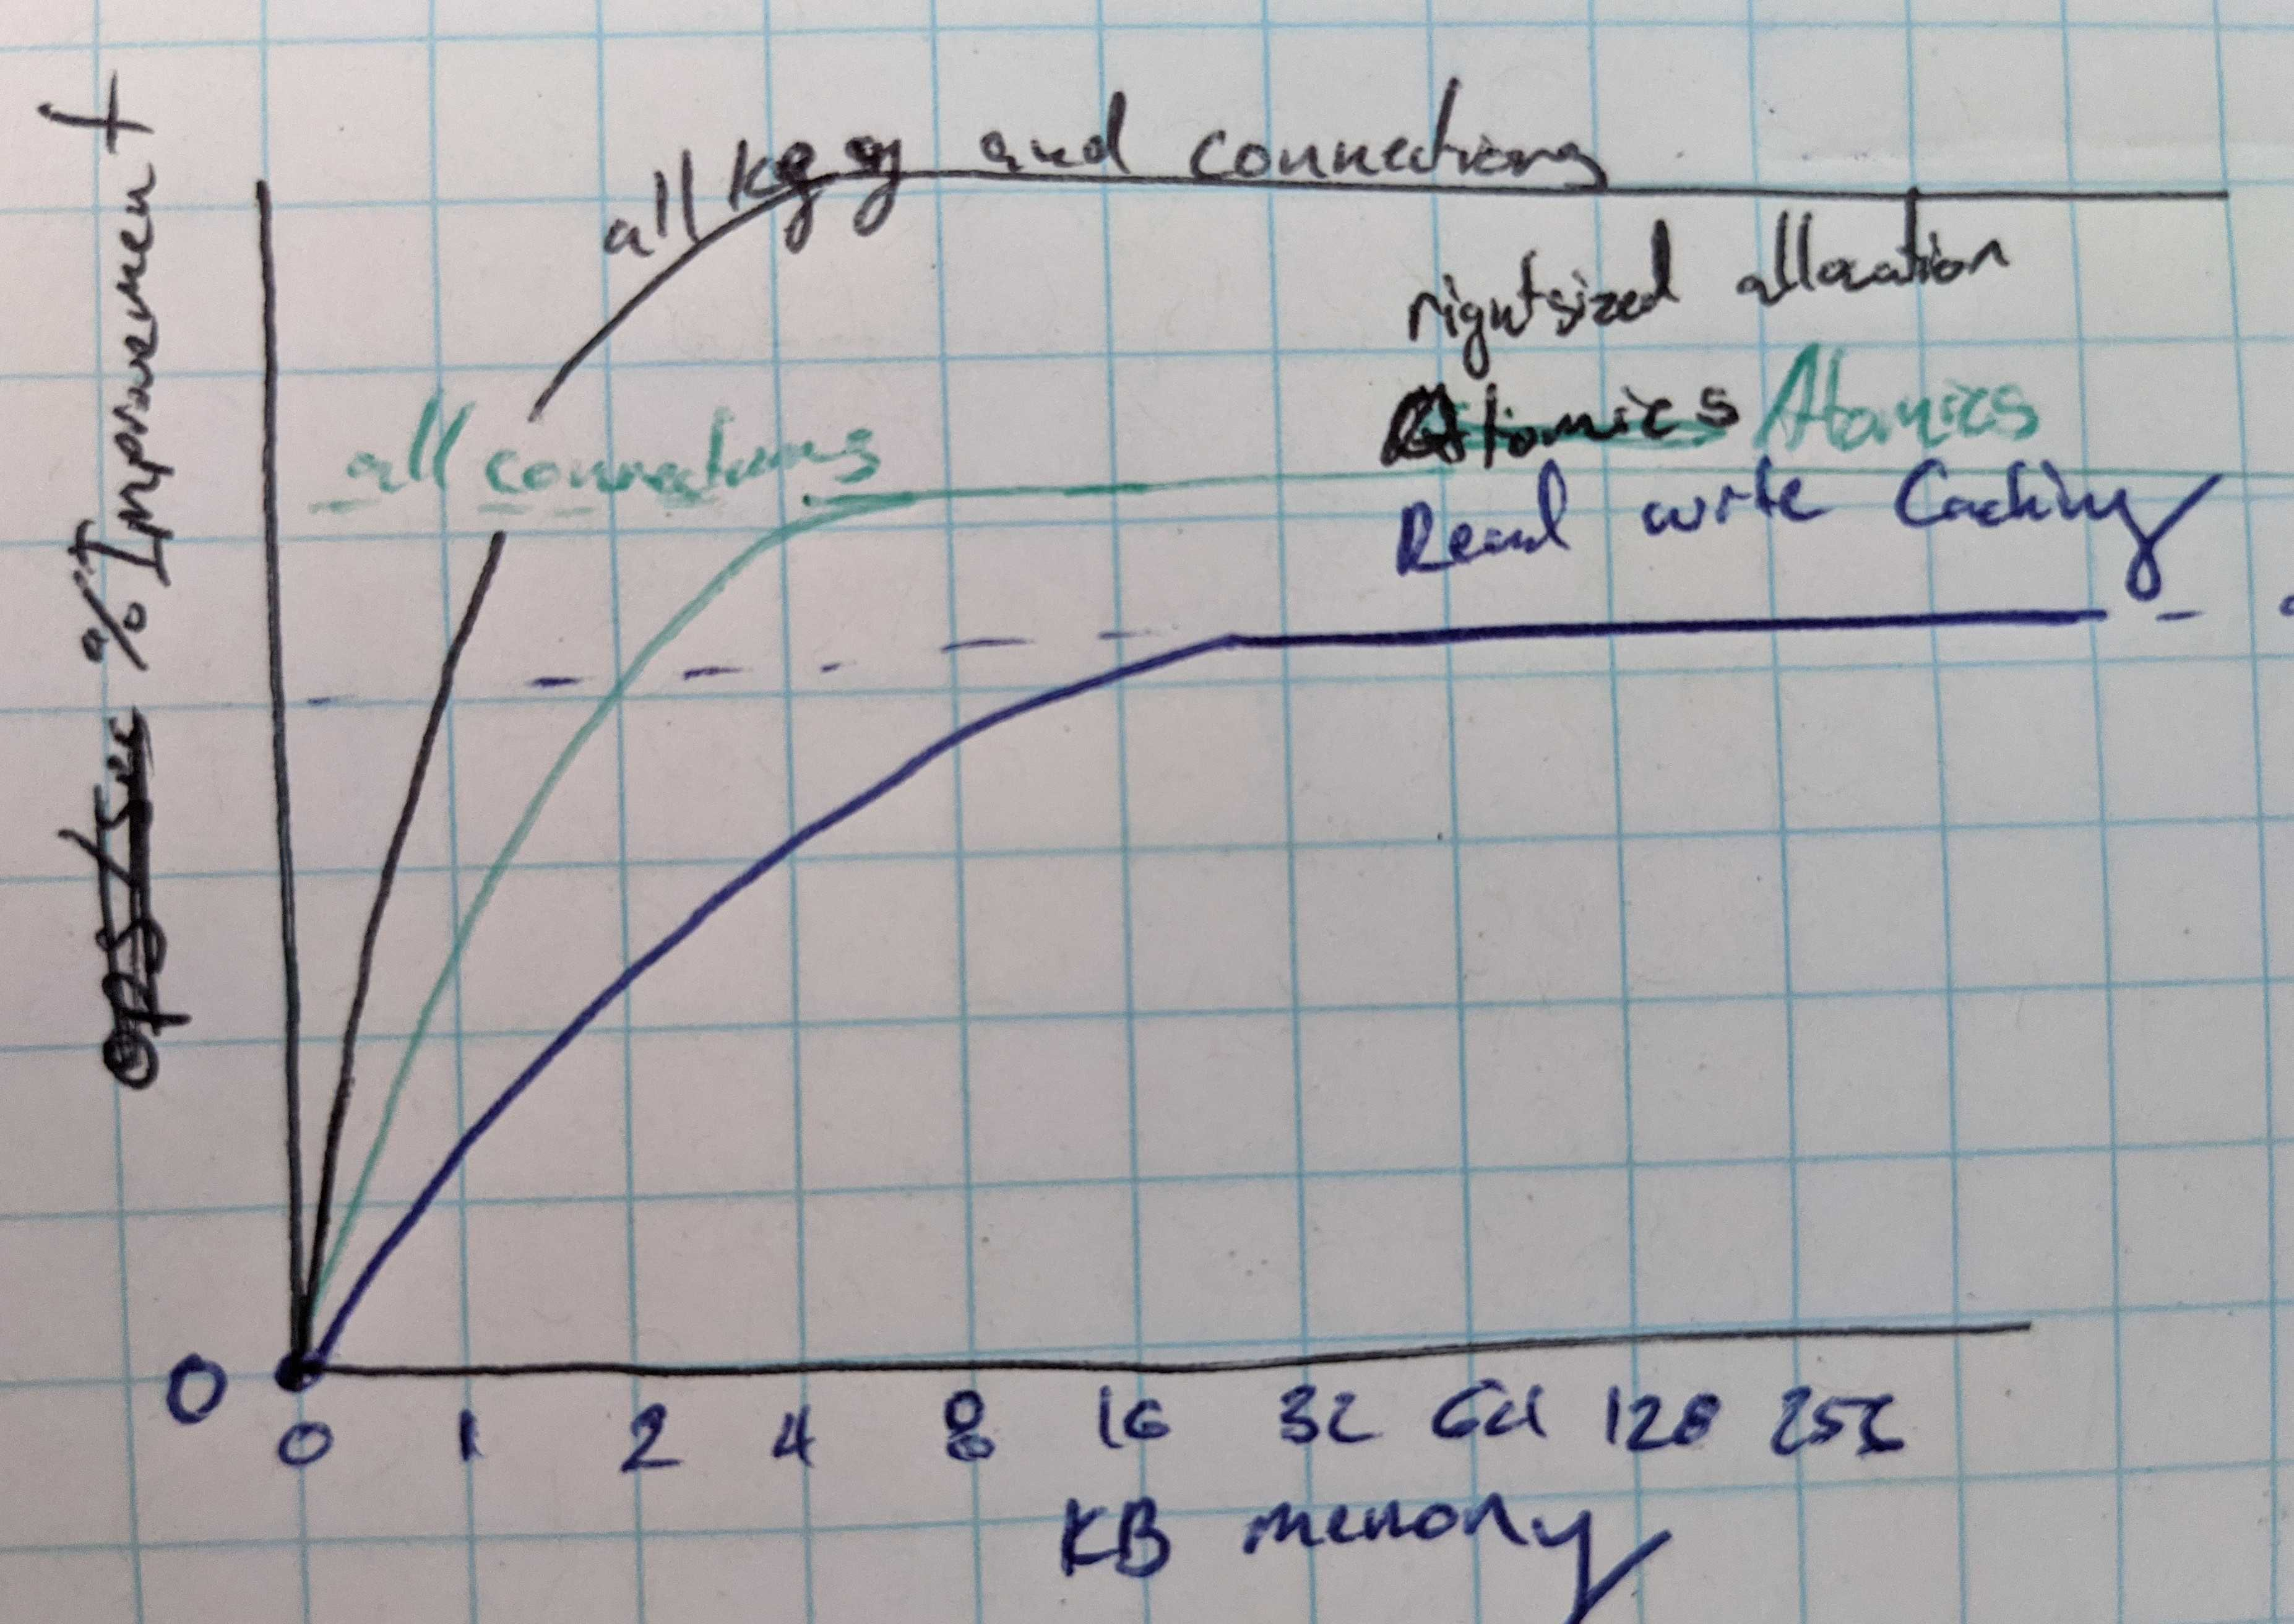
\includegraphics[width=0.45\textwidth]{fig/memory_util.jpg}
%     \caption{{Relative performance improvement of our techniques with restricted amounts of memory. Here a rightsized allocation implies that for the given number of connections we could support, all requests were mapped and reads and writes were cached.}}
%     \label{fig:memory_util}
% \end{figure}
%%\todo{say something real about the the memory utilization takeaways}


\subsubsection{Bandwidth reduction}

\begin{figure}
    \center
  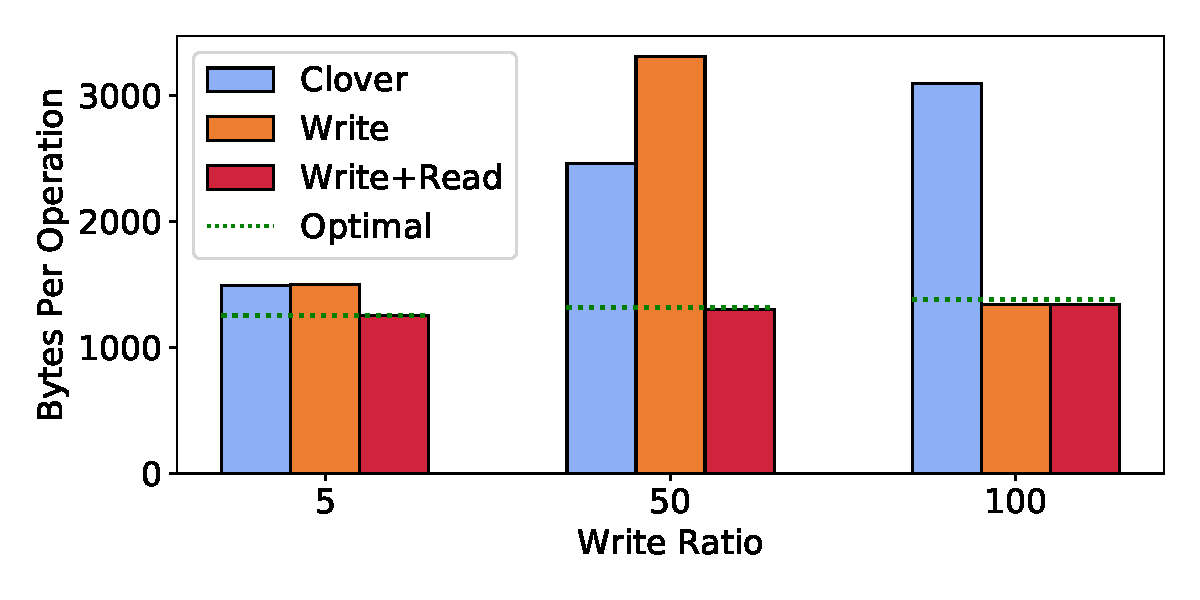
\includegraphics[width=0.99\textwidth]{fig/bandwidth_reduction.pdf}
  \centering
   \vskip -0.5em
    \caption{Average number of bytes required per Clover
      operation on 128-byte objects using each of the three techniques at various write
      intensities.}
    \label{fig:bandwidth_reduction}
     \vskip -0.5em
\end{figure}




%Placing memory operations in-band with regular network traffic can be
%problematic as applications' remote memory usage has the potential to
%vary dramatically per application.
Under contention, Clover's remote operations can require additional
packet exchanges which inflate the bandwidth necessary to service the
same number of memory accesses.  \sword's steering algorithms
remove the need for requests to retry, eliminating the overhead.
%
%Figure~\ref{fig:bandwidth_reduction} shows the average bytes
%per Clover operation under three different workloads for default
%Clover as well as {\sword}'s two steering techniques.
%
%% We calculate the optimal expected cost of a Clover operation by
%% averaging the cost of a successful operation across reads and
%% writes. We get the weighted average by multiplying the cost of a read
%% and write by the appropriate workload percentage. Each write consists
%% of an RDMA write followed by a CAS, along with the responses for each
%% message. A read consists of an RDMA read and read response, and
%% usually an additional metadata read made asynchronously with the main
%% read to fetch the latest position of the tail in case the first memory
%% read fails. Clover performs this second read opportunistically (in
%% around 99 percent of all reads in these workloads), however sometimes
%% it is omitted leading to a small over-approximation in our estimate of
%% ``optimal''.
%
Figure~\ref{fig:bandwidth_reduction} plots the average bytes per
operation for each strategy across the three workloads with writes.
(The read-only workload, not shown, never needs to retry.) We calculate the value
for each technique by summing the total bandwidth across a run and
dividing by the number of operations. Clover's bandwidth usage
increases with contention, growing by 2.5$\times$ at 5\% and
16$\times$ at 50\% writes---all of which is recovered by applying
read and write steering. Write steering alone causes significant
inflation in the cost of operations at 50\% writes because many read
requests fail as discussed above.

\subsubsection{Tail latency}

\begin{figure}
    \center
    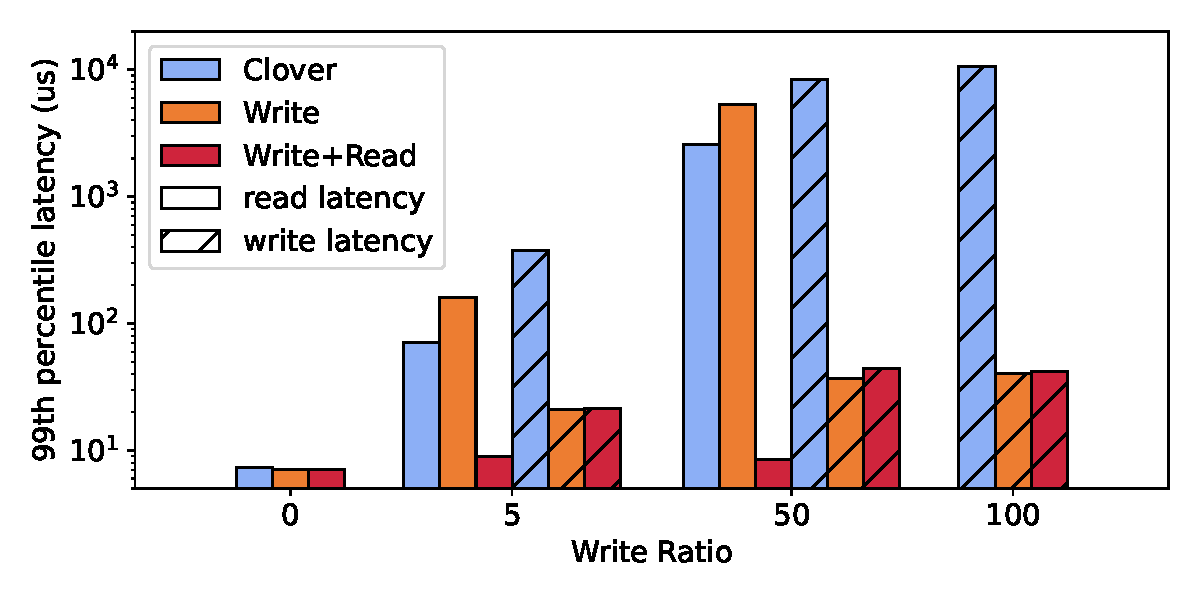
\includegraphics[width=0.99\textwidth]{fig/99th_latency_dense.pdf}
\vskip -0.5em
    \caption{99th-percentile tail latencies of read (solid) and write
      (striped) Clover operations at various write intensities. (Note logarithmic $y$ axis.)}
    \label{fig:tail_latency}
%      \vskip -1em
\end{figure}

%% Perhaps the most critical variable that governs overall system % performance
%is tail latency. In the context of disaggregated memory % systems, reads and
%writes are often deeply integrated into the % computational logic of a program
%and the whole program must wait for a % page fault to complete before
%continuing. We therefore consider poor % tail latency to be a fundamental
%barrier to the widespread adoption of % far memory systems.
Optimistic concurrency is well known to exhibit poor tail latency under
contention, and Clover is no exception.  \sword\ significantly reduces latency
as steering ensures that nearly all requests succeed on the first try.
%
Figure~\ref{fig:tail_latency} shows the 99th-percentile tail latencies
associated with \sword's read and write steering in comparison to default Clover
at varying write intensities. Clover's p99 read latency (solid blue) at 5\%
writes is 70~$\mu$s, around 10$\times$ its baseline our our testbed. With read
and write steering (solid red) the read tail latency drops to 8~$\mu$s---a
8$\times$ improvement over Clover even in this low-contention regime. At 50\%
writes the performance increase from steering increases dramatically: p99 read latency drops by over 300$\times$.
%% As discussed above, in either % case applying write steering alone actually
%hurts performance, as it % makes reads more likely to fail.  % %read
%performance is improves by 2$\times$ % %relative to Clover with the exception
%of write steering alone. When % %write steering is applied without the aid of
%read steering the writes % %quickly out-pace the reads, leading the vast
%majority of reads to fail % %on their first attempt.  % Given that these tests
%were conducted with a % Zipf distribution across 64 cores it is highly likely
%that more than % one thread is writing to the hottest keys at any point during
%the % run. This leads some read requests to fail 10s of times before %
%succeeding.
%
%Because of this property we suggest that read and write steering be used in
%concert unless the workload is explicitly known.
%
Writes (hashed) have slightly more than double the latency of reads as they
require two round trips and atomics are slower to execute than other operations.
Combined write and read steering provides a 17, 189, and 252$\times$ improvement
in write tail latency, respectively, across 5, 50, and 100\% write workloads.
As one might expect, performing write steering alone privileges writes over
reads, dropping their tail latencies slightly further---at the cost of a
dramatic spike in read tail latency.

%% Figure~\ref{fig:tail_latency} also shows the performance of queue pair
%% mapping and atomic replacement (CAS$\rightarrow$Write) when applied in addition
%% to write+read steering.  Because the requests are already likely to
%% succeed, there is no reason to expect any significant drop in tail
%% latency by vectoring the requests to a particular QP or removing the
%% CAS guard.  Rather, these plots show that the (significant) 
%% logic required in {\sword} to implement these functions result in only
%% marginal increase in tail latency relative to steering alone---and still
%% significantly outperforms Clover alone.


%The application of QP mapping and swapping
%CNS to writes does little to effect tail latency as their performance
%cost comes largely as an increase to the average.

\subsubsection{Partial steering}

\begin{figure}
    \center

    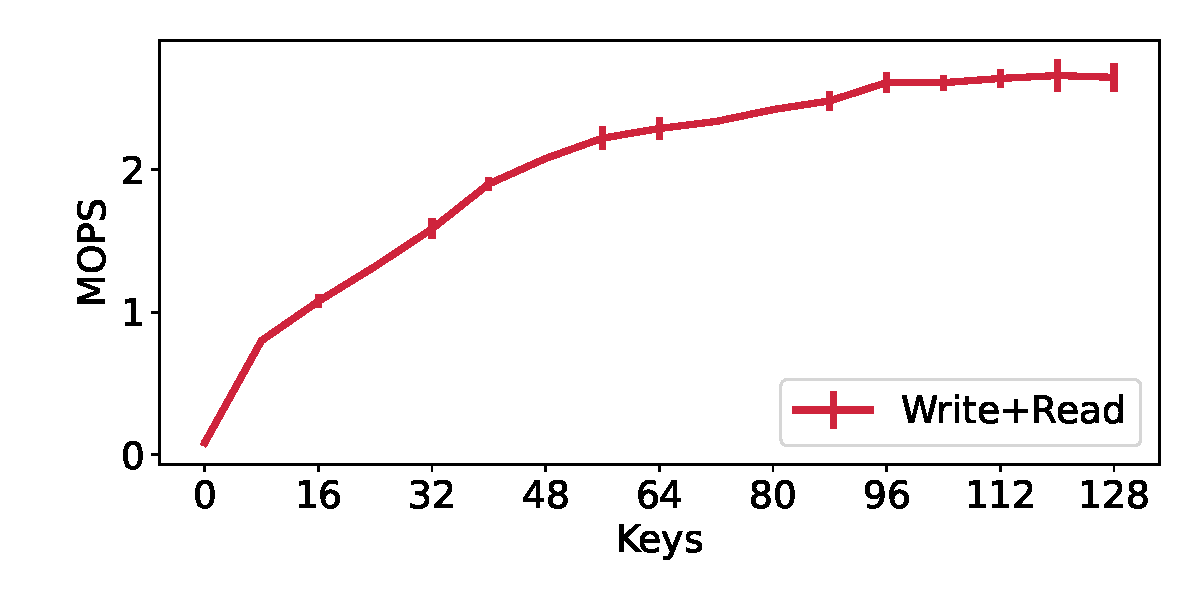
\includegraphics[width=0.99\textwidth]{fig/keys_tracked.pdf}
\vskip -0.5em
    \caption{Per-client throughput as a function of the number of
      Clover keys \sword\ steers.  50:50 workload averaged 
      across 6 hosts each running 56 threads.  }
    \label{fig:keys_tracked}
%      \vskip -1em
\end{figure}

One of most appealing aspects of \sword's steering is the fact that it
need not be applied to all servers, or even memory regions (i.e.,
Clover keys) of a given server.
%In the presence of heavy-tail
%workloads, even steering accesses to a msall number of hot (i.e.,
%highly contended) keys can provide a major performacne boost.
Figure~\ref{fig:keys_tracked} shows per-client throughput as a
function of the number of keys steered by \sword.  To accentuate the
impact, we use a Zipf parameter of 1.5---as opposed to 0.99 in prior
experiments---to enhance the locality of requests.  (See Appendix~\ref{ss:zipf} for a full range.)
%If a programs state is too large to cache on a switch (millions of keys) but a
%few hot keys are highly contested, {\sword} can still provide significant
%benefits by acting on only on the contested state. In the following experiment
%we track a subset of Clovers keys, allowing the rest to flow through
%uninterrupted. In this experiment we run clover at a zipf of 1.5 (most requests
%are on lower keys). We add keys to \sword's tracking list in order of hotness by
Steering requests for only the hottest-8 keys provides a 9.5$\times$
improvement while tracking the hottest 64 delivers
27$\times$.
%; maximum performance boost (i.e., tracking all keys, not shown) is
%(c.f. Figure~\ref{fig:contention}).




\section{Future work}

%\textbf{More data structures}:
%%
While our initial exploration has focused explicitly on Clover and its
append-only key/value chain structure, our approach is not limited to
a particular datastructure nor only associative operations. More
complex structures can be supported, but the choice of structure must
be made with care.  For our caching approach to resolve metadata
conflicts in-network, it requires enough information to enforce remote
datastructure integrity invariants. Invariants such as ordering, or
maintaining a balance in a tree require more metadata and computation
to enforce than appending to the tail of a list. We plan to
investigate data structures which have the ideal property of requiring
a small amount of metadata (ideally $O(\log n)$, or $O(\log\log n)$) to
maintain their structural invariants while also supporting more
operations, such as range queries.

\emph{Design bottlenecks.} As observed during our evaluation,
%%
compare-and-swap operations bottleneck quickly on existing hardware
when locking is applied across queue pairs~\cite{design-guidelines},
limiting the maximum performance of systems that rely on it as a
guard.  We are exploring two potential approaches for reducing
NIC-based lock contention: 1) Remap keys to QPs in flight. Cross-QP
locking can be avoided if all requests to a shared remote memory
address arrive on the same destination QP. 2) Compare-and-swap is not
required for requests handled by our algorithm as they are
serialized. C\&s operations can be converted to writes by replacing a
few RDMA header fields. This approach would allow full-speed operation
throughput with zero locking.


\emph{Resolution interface.}
%%
Designing and running custom code on programmable switches is hard,
while understanding how to resolve write conflicts is relatively
easy. We would like to design a generic interface for developers to
resolve write conflicts, and orchestrate in-flight RDMA operations in
an application-independent fashion, perhaps as part of a larger
disaggregated computing framework or operating system~\cite{legoos}.

\section{discussion}

In this sections we discuss the limitations, generality, and scalability of our approach.



\textbf{RDMA Failures:}
%%
In our approach the switch updates it's memory prior to the RDMA packet
landing in remote memory. This operation is safe under the assumption that no
packets are reordered after egress from the switch and that all operations
are successful. If a c\&s packet updates switch memory, and then is rejected
by the NIC or endhost a reconciliation of memory must take place. The
signifier to the switch that a failure has occurred is an RDMA c\&s NACK. When
this occurs the switch can dump all of it's soft state and reset. This will
cause the clover protocol to revert to it's default chain walk to learn new
values. Our approach requires only a single successful c\&s operation per key
to rebuild its cache.

\textbf{Read acceleration:}
%%
Our current implementation concentrates of fixing write contention,
however there is no limitation which prevents us from gaining a performance
boost on reads. In future work the same RDMA cache can be used to steer
reads which are issued by clients with stale information.


\textbf{Scalability Implications:}
%%
The advantage of using a TOR is that all operations within a rack can be
serialized. However in many cases this degree of total ordering is not
required. For instance access to a single memory server can be serialized by
performing ordering on a SmartNIC connected to the endhost. Our techniques
could be built into smartnics which would allow for them to scale arbitrarily
under the assumption that writes do not span multiple remote memory machines.


\textbf{Alternative Datastructures}
%%
As noted in~\ref{sec:future} the crux of applying our approach to other
structures is the complexity of the data structures invariants. For Clover
the invariant is simple, all writes must append to the end of the list. To
enforce this invariant the last element of the list must be cached to ensure
that the tail location is known.

The more complicated the structural invariants are to maintain, the greater
the information which must be cached; for example an \textit{ordered} list.
To illustrate the additional complexity of maintaining order consider how
clients could perform inserts. First, like clover, clients could write their
entry to a private memory region. Second two pointers must be written, one
which points to the next item, and another from the prior item to the newly
written one. The client could issue the writes itself, however when the
insert occurs it would need to traverse part of the list to ensure that the
result had been inserted to the correct location and collect a lock on both
the prior and successor items. Enforcing the ordering invariant requires that
the switch cache the entire list.

Ordering is more complex in terms of space to maintain compared to only
appending to a lists tail. The complexity of generalizing our technique to
any data structure being is that the switch must cache all necessary metadata
to maintain a data structures invariants.

We've considered exploring the class of data structures which have either
weak structural invariants, or those which only cost $O(1)$ to check. Additionally some
data structures amortize the cost of operations which require complex
invariants. For instance, rather than storing an ordered list, using a
partially ordered list with fast accesses which can be periodically
transformed with expensive operations to be consistent.

%We are exploring the potential set of future data structures currently. One
%example of a data structure with more complex invariants is a B-Tree. In this
%case ordering must be persevered at each level of the tree, and also some
%operations require that many locks up the tree be obtained. We speculate that
%algorithms used in Clover such as writing to a local scratch space and then
%atomically updating a shared vairable could be used in more complicated
%scenarios as well, such as this.

%\textbf{zipfan 0.75} 
%%
%We chose this because it shows scaling isues before we
%start to hit the hardware issues. There is no good answer to this question.

%\textbf{Why does the switch have to store the last key written per client}
%%
%The last write is not stored. Client writes occur in two parts, a private
%write to their own scratch space, and a commiting atomic c\&s. The write
%which is stored is the outstanding writes, i.e writes which have been placed
%in the local storage, but not yet connected via a commiting operation.













\balance
\vspace{-0.3cm}
{\footnotesize \bibliographystyle{acm}
\bibliography{paper}}
\vspace{-0.5cm}

\end{document}
